\setcounter{section}{0}
%\setcounter{propositions}{0}


\begin{center}
 {\large \textbf{Appendix}}
\end{center}



\emph{
In the supplementary material,
we first show more visualizations to understand the predicted filter flows,
then show if it is possible to refine the results
by iteratively feeding deblurred image to the same model
for the task of non-uniform motion blur removal.
We finally present more qualitative results for all the three tasks studied in this paper.
}





\section{Visualization of Per-Pixel Loading Factors}

As a supplementary visualization to the principal components by PCA shown in the main paper,
we can also visualize the per-pixel loading factors corresponding to each principal component.
We run PCA over testing set and show the first six principal components and the corresponding
per-pixel loading factors as a heatmap in Figure~\ref{fig:demo_loadingFactorPCA}.
With this visualization technique,
we can know what region has higher response to which component kernels.
Moreover,
given that the first ten principal components capture $\ge 99\%$ filter
energy (stated in the main paper),
we expect future work to predict compact per-pixel filters using low-rank technique,
which allows for incorporating long-range pixels through large predictive filters while
with compact features (thus memory consumption is reduced largely).





\begin{figure}[t]
    \centering
    \begin{minipage}{0.49\textwidth}
        \centering
        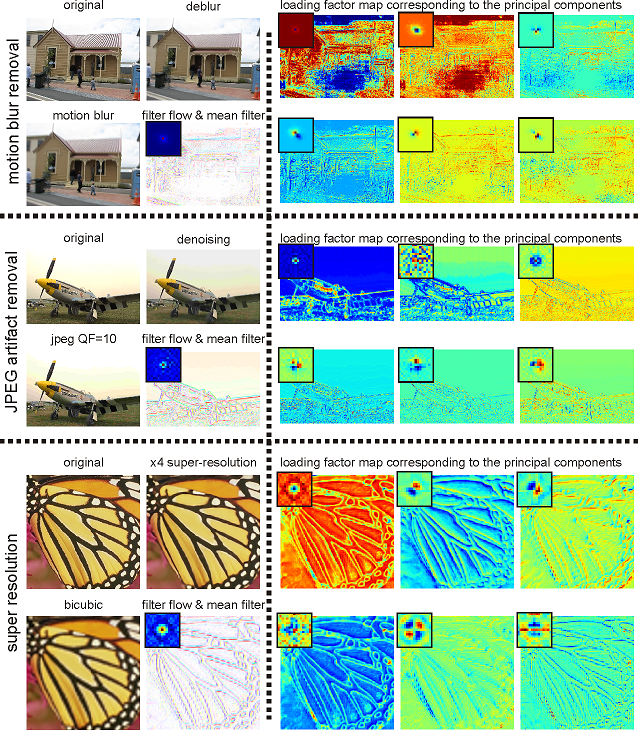
\includegraphics[width=1\linewidth]{demo_analysisFF_v2.png}
        %\captionsetup{width=0.999\textwidth}
    \end{minipage}
    \caption{
    We show the original image,
    low-quality input and the high-quality output by our model as well as the mean kernel and filter flow maps on the left panel,
    and the first six principal components and the corresponding loading factors as heatmap
    on the right panel.
    Best seen in color and zoom-in.}
    \label{fig:demo_loadingFactorPCA}
\end{figure}


\section{Iteratively Removing Motion Blur }
As the deblurred images are still not perfect,
we are interested in studying if we can improve performance by iteratively running the model, i.e.,
feeding the deblurred image as input to the same model one more time to get the result.
We denote this method as PFF+1.
Not much surprisingly,
we do not observe further improvement as listed in
Figure~\ref{tab:compare_motion_deblur_more}, instead,
such a practice even hurts performance slightly.
The qualitative results are shown in Figure~\ref{fig:iterativeRefine},
from which we can see the second run does not generate much change through the filter flow maps.
We believe the reason is that,
the deblurred images have different statistics from the original blurry input,
and the model is not trained with such deblurred images.
Therefore, it suggests two natural directions as future work for improving the results,
1) training explicitly with recurrent loops with multiple losses to improve the performance,
similar to~\cite{belagiannis2017recurrent,li2016iterative,romera2016recurrent,
kong2017recurrentSceneParsing,kong2018pixel},
or 2) simultaneously inserting an adversarial loss to force the model to hallucinate
details for realistic output, which can be useful in practice as done in~\cite{ledig2017photo}.


{
\setlength{\tabcolsep}{0.9em} % for the horizontal padding
\begin{table*}[t]
\centering
%\hspace{-1mm}
\caption{Comparison on motion blur removal over the non-uniform
motion blur dataset~\cite{bahat2017non}. PFF+1 means we perform PFF one more time by taking
as input the deblurred image by the same model. }
\vspace{-1mm}
%\footnotesize
%\scriptsize
%\small
\begin{tabular}{l c c c c c c c c c c c c c} % >{\centering}m{1cm}
\hline\hline
    & \multicolumn{6}{c} {\texttt{Moderate Blur}}  \\
    \cmidrule(r){2-7}
    metric & \cite{xu2013unnatural} &  \cite{sun2015learning} &  \cite{bahat2017non} & CNN
    & {\bf PFF}
    & PFF+1 \\
    %& PFF$_{ft}$+1 \\
    \hline
PSNR        & 22.88 & 24.14 & 24.87 & 24.51 & {\bf 25.39}  & 25.28  \\
SSIM        & 0.68  & 0.714 & 0.743 & 0.725 & {\bf 0.786}  & 0.783  \\
\hline
&  \multicolumn{6}{c} {\texttt{Large Blur}}    \\
\cmidrule(r){2-7}
    metric & \cite{xu2013unnatural} &  \cite{sun2015learning} &  \cite{bahat2017non} & CNN
    & {\bf PFF}
    & PFF+1 \\
    %& PFF$_{ft}$+1  \\
    \hline
PSNR        & 20.47 & 20.84 & 22.01 & 21.06 & {\bf 22.30}  & 22.21  \\
SSIM        & 0.54  & 0.56  & 0.624 & 0.560 & {\bf 0.638}  & 0.633  \\
\hline\hline
\end{tabular}
%\hspace{0.5mm}
\label{tab:compare_motion_deblur_more}
%\vspace{-1mm}
\end{table*}
}


\begin{figure*}[t]
    \centering
    \begin{minipage}{0.95\textwidth}
        \centering
        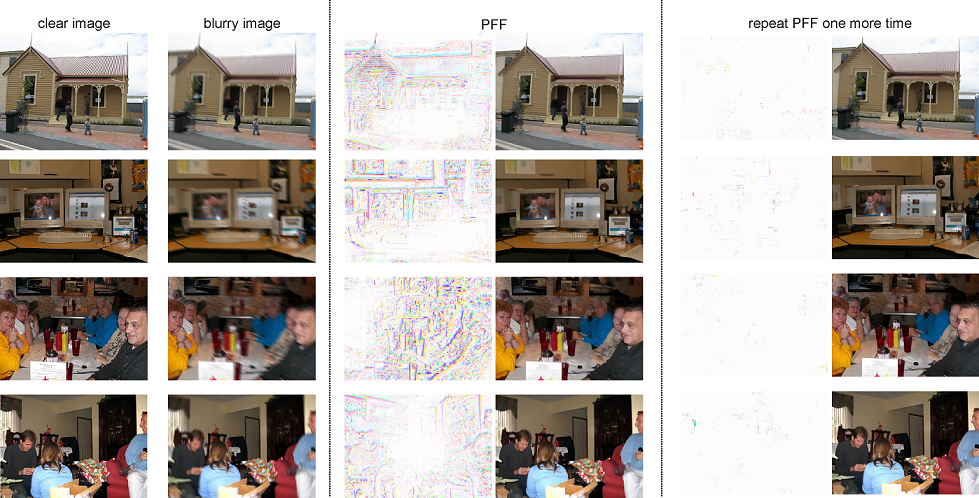
\includegraphics[width=1\linewidth]{iterativeRefine.png}
        %\captionsetup{width=0.999\textwidth}
    \end{minipage}
    \caption{
    We show deblurring results over some random  testing images from the dataset released by~\cite{bahat2017non}.
    We first feed the blurry images to PFF model, and obtain deblurred images;
    then we feed such deblurred images into the same PFF model again to see if this iterative practice refines
    the output.
    However,
    through the visualization that iteratively running the model changes very little as seen
    from the second filter flow maps.
    This helps qualitatively explain why iteratively running the model does not improve deblurring performance
    further.
    }
    \label{fig:iterativeRefine}
\end{figure*}



\section{More Qualitative Results}

In Figure~\ref{fig:more_motionblur}, \ref{fig:more_JPEG_reduction} and \ref{fig:more_SISR},
we show more qualitative results for
non-uniform motion blur removal,
JPEG compression artifact reduction
and single image super-resolution, respectively.
From these comparisons and with the guide of filter flow maps,
we can see at what regions our PFF pays attention to and how it outperforms
the other methods.




\begin{figure*}[t]
    \centering
    \begin{minipage}{0.97\textwidth}
        \centering
        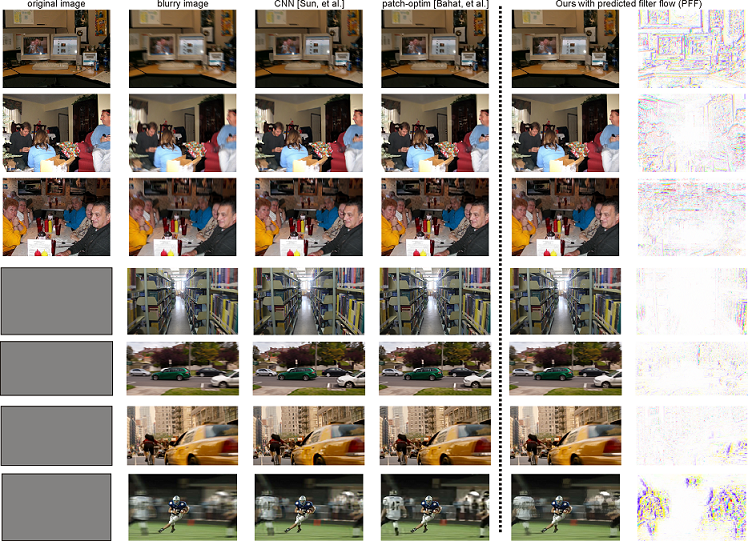
\includegraphics[width=1\linewidth]{supple_blur.png}
        %\captionsetup{width=0.999\textwidth}
    \end{minipage}
    \caption{Visual comparison of our method (\emph{PFF}) to \emph{CNN [Sun, et al.]}~\cite{sun2015learning} and
    \emph{patch-optim [Bahat, et al.]}~\cite{bahat2017non}
    on more testing images released by~\cite{bahat2017non}.
    Please be guided with the strong edges in the filter flow maps to compare visual details in the deblurred images by different methods.
    The last four rows show real-world blurry images without ``ground-truth'' blur.
    Note that for the last image,
    there is very large blur caused by the motion of football players.
    As our model is not trained on larger kernels which should be able to cover the size of blur,
    it does not perform as well as \emph{patch-optim [Bahat, et al.]}~\cite{bahat2017non}.
    But it is clear that our model generates sharp edges in this task.
    Best view in color and zoom-in.}
    \label{fig:more_motionblur}
\end{figure*}



\begin{figure*}[t]
    \centering
    \begin{minipage}{0.97\textwidth}
        \centering
        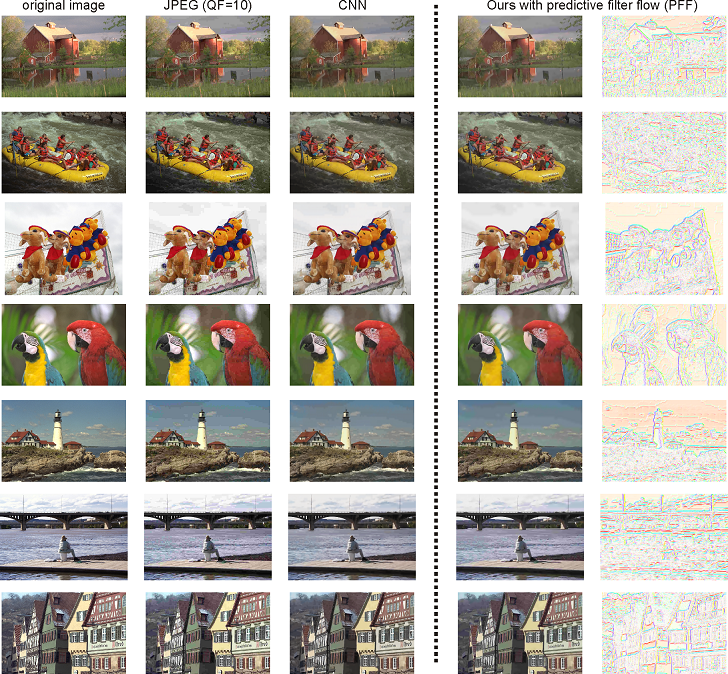
\includegraphics[width=1\linewidth]{supple_jpeg.png}
        %\captionsetup{width=0.999\textwidth}
    \end{minipage}
    \caption{
    Visual comparison between CNN and our method (\emph{PFF}) for JPEG compression artifact reduction.
    Here we compress the original images using JPEG method with quality factor (QF) as 10.
    Best view in color and zoom-in.}
    \label{fig:more_JPEG_reduction}
\end{figure*}



\begin{figure*}[t]
    \centering
    \begin{minipage}{0.77\textwidth}
        \centering
        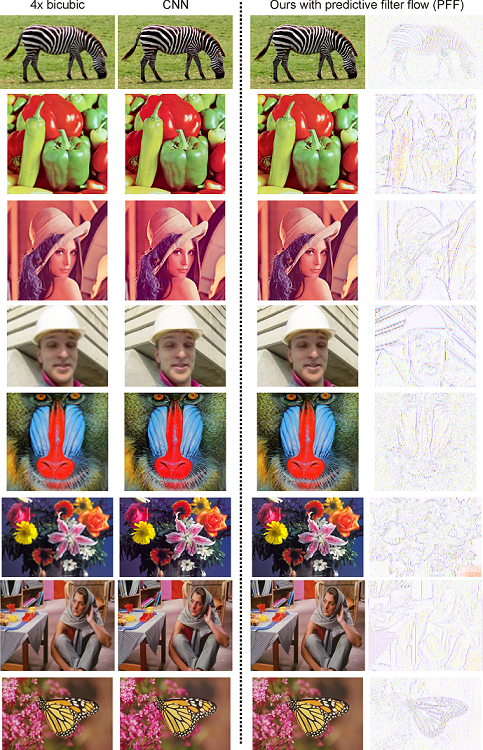
\includegraphics[width=1\linewidth]{supple_sisr.png}
        %\captionsetup{width=0.999\textwidth}
    \end{minipage}
    \caption{
    Visual comparison between CNN and our method (\emph{PFF}) for single image super-resolution.
    Here all images are super-resolved by 4$\times$ larger.
    We show in the first column the results by bicubic interpolation.
    Best view in color and zoom-in.}
    \label{fig:more_SISR}
\end{figure*}

